\documentclass{article}
\usepackage{url}
\usepackage{mathtools}
\usepackage{tikz}
\usetikzlibrary{arrows,positioning}
\begin{document}
\title{Ripple Consensus Review}
\author{Peter Todd}
\date{FIXME}
\maketitle

\section{Activities performed}

The Ripple consensus review investigation had four major activities associated
with it:

\begin{enumerate}

    \item Reviewed whitepapers and development documentation at ripple.com

    \item Reviewed existing third-party critism.

    \item Setup and run a full node.

    \item Reviewed C++ implementation, specifically the 0.27.4 tag.\footnote{git commit 92812fe7239ffa3ba91649b2ece1e892b866ec2a}

\end{enumerate}


\section{Overall architecture}

Ripple has diverged significantly from the original concept of a decentralized
network representing money explicitly as debt relationship between
parties.\cite{btcmag-introducing-ripple} While the concept of a debt
relationship still exists in the form of trust lines between participants, the
bulk of the codebase and developer documentation now focuses\footnote{For
    instance the ``Tutorials'' section of the Ripple website only explains how
    to create transactions that modify the ledger; there is almost no information
available on how to actually use the trustlines feature.} on the use and
maintenance of a global ledger of transactions and account balances.
Additionally a native currency, XRP, has been added, which is used for
anti-spam transaction fees\footnote{A small amount of XRP is irrovocably
destroyed for every transaction.}, as well as to serve as a universal currency.


\subsection{Hashing and serialization}

Though various parts of the Ripple user API's and networking use industry
standard serialization formats like JSON and Google Protobuf, for
consensus-critical functionality Ripple uses a custom tag-length-value
serialization and hashing scheme. This is not unexpected as industry standard
serialization schemes rarely, if ever, account for the need to create hash
digests from represented objects.

\begin{equation}
    \textit{Serialize}(\text{obj}) = t_0 n_0 d_0 + \hdots + t_n n_n d_n
\end{equation}

Hashing of objects generally uses the following scheme, implemented by
STObject::getHash(), resulting in a $256\text{bit}$ digest:

\begin{equation}
    H(\text{obj}) = \text{SHA512}(p + \text{Serialize}(\text{obj}))[0:256\text{bits}]
\end{equation}

The prefix $p$ is per-object-type, guaranteeing that objects of different types
will always have a different hash.\footnote{This is commonly known as
\emph{tagged hashing} in the literature.} For objects containing signatures,
such as transactions, there is a similar but separate \emph{signing hash}
implemented by the function STObject::getSigningHash(). Unlike the standard
hash, the signing hash does not serialize signature fields.


\subsection{Transactions}

Unlike Bitcoin, transactions increment and decrement account balances; they do
not directly consume the output of other transactions. To prevent replay
attacks accounts and transaction have sequence numbers; a transaction is only
valid if the Sequence number is exactly one greater than the last-valided
transaction from the same account. Additionally an optional AccountTxnID field
is available for use within transactions; the transaction is only valid if the
sending account's previously-sent transaction matches the provided hash.

Authentication is performed with a simple signature scheme; a scripting system
is not available, nor is multisignature support. To implement the latter a
highly complex single-purpose scheme\cite{ripple-wiki-multisign} has been
proposed.


\subsection{Ledger}

Information on the exact structure of the Ripple ledger is somewhat spotty.

how exactly does the skiplist work?


\subsection{Unique Node List}

The actual process of determining what version of the ledger is correct starts
with the Unique Node Listi, (UNL) a list of public keys meant to be associated
with active nodes the node operator believes are
``unique''.\cite{ripple-wiki-unl} Ripple Labs suggests that UNL's ``should have
100+ nodes on them.''\cite{ripple-wiki-unl} and provides a ``starter'' UNL at
\url{https://ripple.com/ripple.txt} with $5$ to $8$ nodes.\footnote{Exactly how this UNL is
generated is unknown; the author downloaded it on multiple occasions getting
between $5$ to $8$ nodes each time, mostly the same.}

Through the Ripple Protocol Consensus Algorithm\cite{ripple-consensus-paper}
nodes on the UNL vote to determine the contents of the Ripple ledger. While the
actual protocol contains a number of rounds of proposals and voting the end
result can be described as basically a supermajority vote: a transaction is
only approved if $80\%$ of the UNL of a server agrees with
it.\cite[3.2]{ripple-consensus-paper} Put another way, if $20\%$ of the UNL
choose to reject a transaction, it will not be included in the ledger.

Different nodes may chose to use different UNLs; if the UNLs do not
sufficiently overlap global consensus is not guaranteed because different UNL
``cliques'' can come to consensus independently of each other. For instance
Figure \ref{fig:unl-clique-disjoint} shows a simple example with two UNL
cliques, red and blue, that have forked because of insufficient connectivity,
resulting in the forked blockchain shown in Figure \ref{fig:unl-clique-disjoint-blockchain}.

Increasing the connectivity past the $20\%$ threshold, as shown in Figure
\ref{fig:unl-clique-consensus}, brings both cliques into agreement. However
what happens to the blockchain? The Ripple Protocol Consensus Algorithm paper
is unclear on this point. For instance, the loss and restoration of
connectivity may have been associated with network latency. The paper does
state that "nodes who’s latency grows larger than a preset bound $b$ are
removed from all UNLs"\cite[3.4.1]{ripple-consensus-paper} but does not say if
this removal is meant to be permanent\footnote{In the existing implementation
restarting the node does reload the UNL set from the config file.} nor if by
``all'' they refer to removal from UNLs on all nodes in the network.
Additionally while the author did not have sufficient time to investigate this
point fully, the source code doesn't appear to have any provision for
reorganizations of the ledger when a longer fork is detected.

Regardless, it is certain that following a fork caused by disjoint UNL cliques
the losing side simply has to discard some or all history, as seen in Figure
\ref{fig:unl-clique-post-fork}, possibly resulting in double-spends and
associated financial losses.

\begin{figure}
    \centering
    \includegraphics{figures/unl-clique-disjoint.eps}
    \caption{Disjoint UNL}
    \label{fig:unl-clique-disjoint}
\end{figure}

\begin{figure}
    \centering
    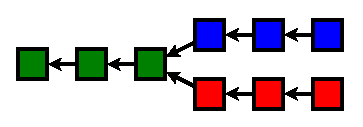
\includegraphics{figures/unl-clique-disjoint-blockchain.eps}
    \caption{Forked blockchain}
    \label{fig:unl-clique-disjoint-blockchain}
\end{figure}

\begin{figure}
    \centering
    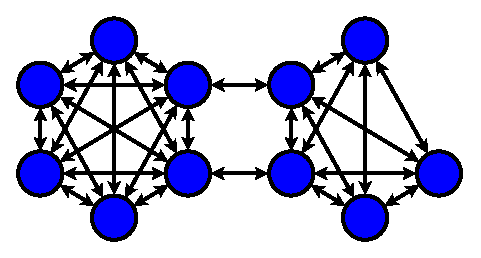
\includegraphics{figures/unl-clique-consensus.eps}
    \caption{UNL cliques in consensus}
    \label{fig:unl-clique-consensus}
\end{figure}

\begin{figure}
    \centering
    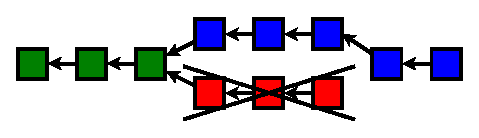
\includegraphics{figures/unl-clique-reorganized-blockchain.eps}
    \caption{Post-fork reorganization}
    \label{fig:unl-clique-post-fork}
\end{figure}



Similarly for a UNL of $n$ nodes it would
take $(4n + 1)/5$ Byzantine failures for an incorrect transaction to be
confirmed.



Claims from ripple: consensus protocol\cite{ripple-consensus-paper} will maintain correctness so long as $f
\le (n-1)/5$ where $f$ is the number of Byzantian failures. However default UNL
list is just $5$ entries, thus $f \le (5-1)/5 = 0.8$ - no failures can be
tolerated.

Put antoher way, you only need to compromise $20\%$ of the nodes in the UNL to
censor a transactions/freeze funds. "failure to agree is agreement to defer"


Is there incentive to use anything but the default UNL? Remember that if you
choose a UNL more than $80\%$ different than others, you can be attacked on
that basis; your full node determines validity of transactions anyway. e.g. the
"add 1000 validators to UNL list" suggestion.

mixing structure: if tx A is rejected, dependent txs are all rejected; will
likely soon result in situation where you can't use different UNL


The Ripple consensus algorithm starts with a Unique Node List. 


what happens with UNL majority is not reached?

test: add extra entries to UNL list, see if ledgers close, if they don't think we know threshold


\section{Attacks}

reference c3 criteria?

big picture with attacks is there is not a minimum cost to them unlike PoW

evaluate attacks for denial-of-service and theft potential; evaluate minimum
cost to carry out attack; possible minimum manpower to carry out attack


Type of attack: DoS and/or theft

Minimum cost: $0, $1k, $10k, $100k

Scope: targetted, broad, global
Duration: hours, days, weeks, indefinite - How long will it take to fix the bug?

we don't attempt to put a dollar figure on harm done, as depends enormously on
how people use ripple


\subsection{Consensus Split}

1) exploit consensus failure.

DoS: Cost \$0, Scope: global, Duration: hours
Theft: Cost \$1k, Scope: varies, Duration: hours

not as synergistic with other attacks; obvious flaw that will be fixed;
time-limited attack


\subsection{Scalability}

DoS: Cost \$100k, Scope: global, Duration: weeks

simply produce a lot of txs, paid for via fees, either covertely or overtly.
System will fail, guaranteed.


\subsection{UNL: Jurisdictional}

DoS/Theft: Cost \$100k, Scope: varies, Duration: indefinite

centralization attack - legal attack against centralized UNL. note
jurisdictional issues with delegating consensus to UNL

biggest issue is how can ripple compete against systems without the global
consensus req? if I'm a bank in russia, why use ripple when it opens me to UNL
issues?


\subsection{Software backdoor}

DoS/Theft: Cost \$0, Scope: varies, Duration: varies

mention unsigned code here


\subsection{UNL: key theft}

prep: Cost \$0, Scope: global, Duration: N/A

Gain control of UNL signing keys through theft/compromise. 


\subsection{History simulation}

Theft: Cost \$0, Scope: targetted, Duration: weeks

from proof-of-stake terminology; simulated history is costless as no work
expended.

use backdoored software as example of how this can happen; also can happen with
jurisdictional attacks

if rippled sees two versions of history, what happens?

rewrite history attack - note lack of cost to rewrite because no PoW; single
implementation so likely we can hack all nodes at once

proof-of-work has a hard bound on rewrite attacks, because can't break laws of
physics

can talk about how cost to do a simulation attack is PoW targets; talk about slasher rule


\section{Synergistic Attacks}

do a directed graph of likely synergistic attack sequences


\bibliographystyle{plain}
\bibliography{paper}

\end{document}
